\subsection{etn.go}

The main structures in "ent.go" are Encoder and Decoder. The first one writes encoded values inside its []byte buffer buf and keeps track of the encoded elements by an index (integer that stores the number of encoded elements) and an addrToIndex map (which takes as key the address of the element that has to be encoded, and as value the current number of encoded elements and the type of the current element). The second one reads from its []byte buffer buf the encoded values and decodes them into ETN valid types (described above) keeping track of the decoded elements types into an indexToValue array.

Constructors:

\begin{itemize}

	\item \emph{func NewEncoder(io.Writer) *Encoder}\\
	Given a io.Writer returns the address of a new Encoder structure.
	
	\item \emph{func NewDecoder(io.Reader) *Decoder}\\
	Given a io.Reader returns the address of a new Decoder structure.

\end{itemize}

Methods of Encoder (the exported ones start with capital letter):

\begin{itemize}

	\item \emph{func (e *Encoder)  Encode(interface{}) os.Error}\\
	Wrapper for EncodeValue(), given an element of generic type (an empty interface in Go can be of any type and can implement any method) encodes that element and returns an os.Error if the element type is not supported.
	
	\item \emph{func (*Encoder) EncodeValue(reflect.Value) os.Error}\\
	Given a generic element (reflect.Value is the reflection interface to a Go value) encodes it using encode() and returns an os.Error if the element type is not supported.
	
	\item \emph{func (*Encoder) encode(reflect.Value)}\\
	Given a generic element encodes it following the rules described in Section 1.
	
	\item \emph{func (*Encoder) u?int[8|16|32|64](u?int[8|16|32|64])}\\
	Given a u?int[8|16|32|64] encodes it writing it into the Encoder []byte buffer using little endian notation (least significant byte is stored in the smallest address).
	
	\item \emph{func (*Encoder) string(string)}\\
	Given a string, writes first its length (encoded as uint32) and then the string into the Encoder []byte buffer. First encodes the length (using \emph{func (*Encoder) length(uint32)}), then encodes the string.
	
	\item \emph{func (*Encoder) write([]byte)}\\
	Given an array of bytes, writes that array using its writer io.Writer.
	
	\item \emph{func (*Encoder) length(uint32)}\\
	Given a length in uint32 the method calls \emph{(*Encoder) uint32(uint32)} to encode the length of an array, slice, map, string.

\end{itemize}

Methods of Decoder (the exported ones start with capital letter):

\begin{itemize}

	\item \emph{func (*Decoder) Decode(interface{}) os.Error}\\
	Wrapper for DecodeValue(), given an element of generic type (an empty interface in Go can be of any type and can implement any method) decodes that element and returns an os.Error if the element type is not supported.
	
	\item \emph{func (*Decoder) DecodeValue(reflect.Value) os.Error}\\
	Given a generic element (reflect.Value is the reflection interface to a Go value) decodes it using decode() and returns an os.Error if the element type is not supported.
	
	\item \emph{func (*Decoder) decode(reflect.Value)}\\
	Given a generic element decodes it following the rules described in Section 1.
	
	\item \emph{func (*Decoder) u?int[8|16|32|64]() u?int[8|16|32|64]}\\
	Decodes a u?int[8|16|32|64] reading it from the Decoder []byte buffer (using little endian notation) and returns the decoded u?int[8|16|32|64] value.
	
	\item \emph{func (*Decoder) string() string}\\
	Decodes a string reading it from the Decoder []byte buffer. First decodes the length (using \emph{func (*Decoder) length() uint32}), then decodes the string.
	
	\item \emph{func (*Encoder) read([]byte)}\\
	Given an array of bytes, reads that array using its reader io.Reader.
	
	\item \emph{func (*Decoder) length() uint32}\\
	Calls \emph{(*Decoder) uint32()uint32} to decode the length of an array, slice, map, string.

\end{itemize}

\begin{figure}[H]
\centering
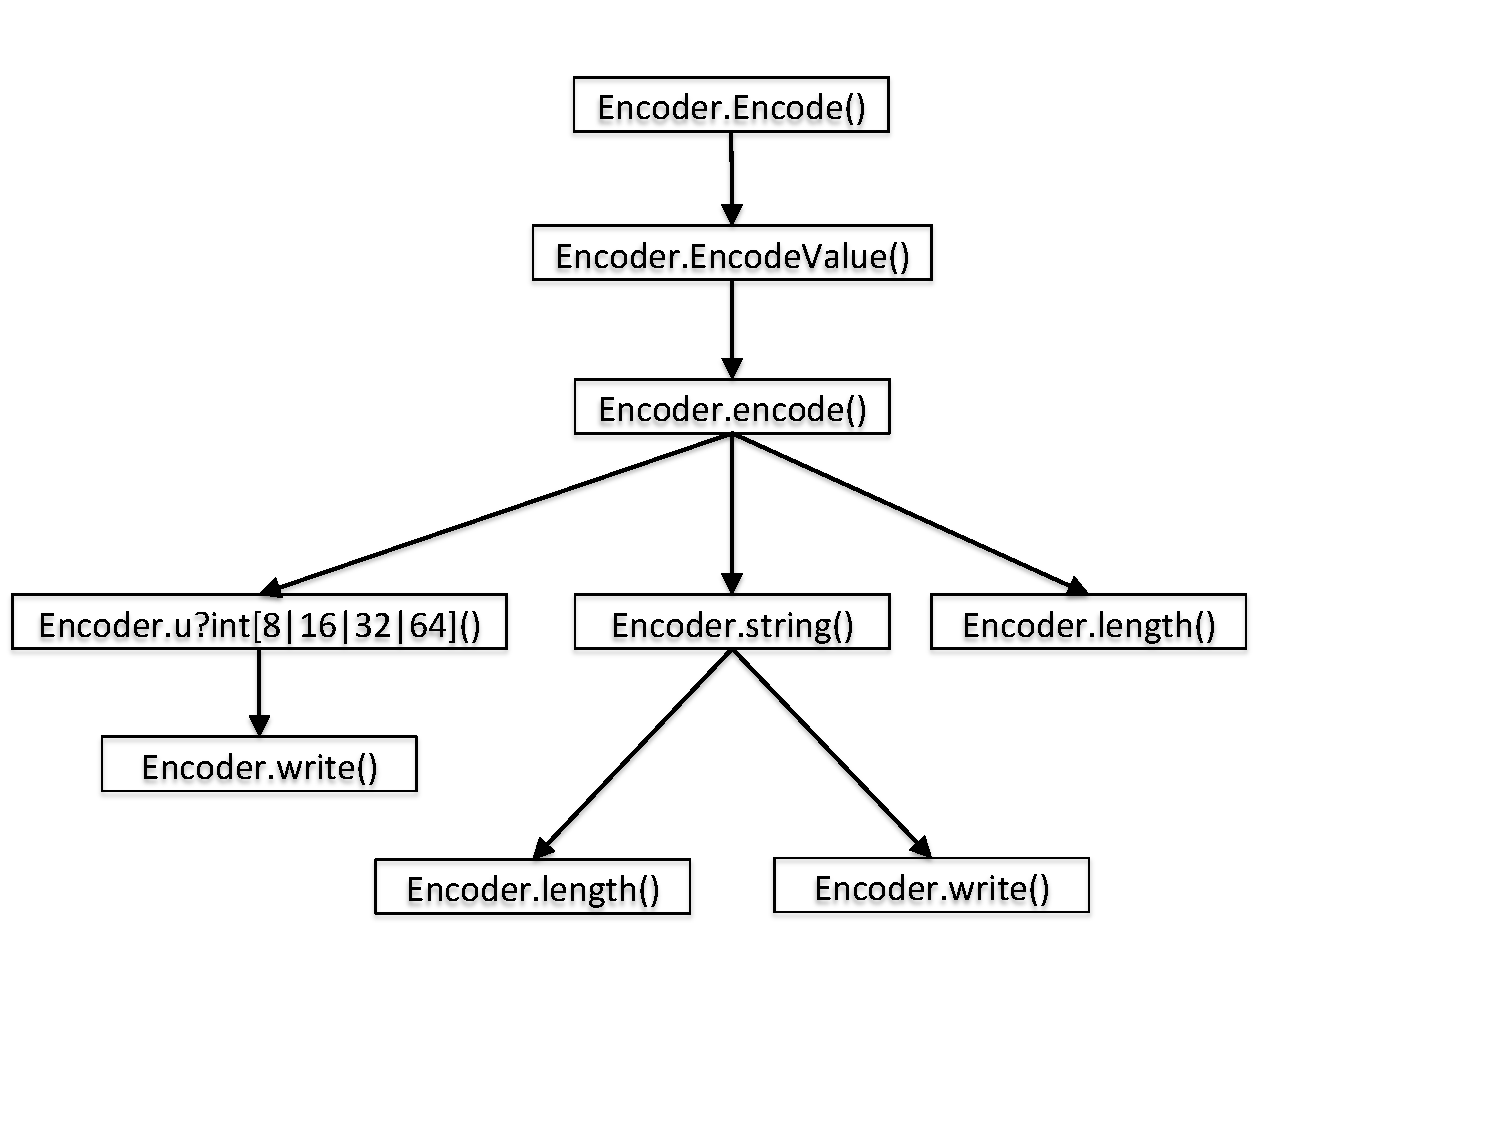
\includegraphics[scale=0.50]{callGraphs/etnEncoderPackage}
\caption{etn.go package: Encoder}
\end{figure}

\begin{figure}[H]
\centering
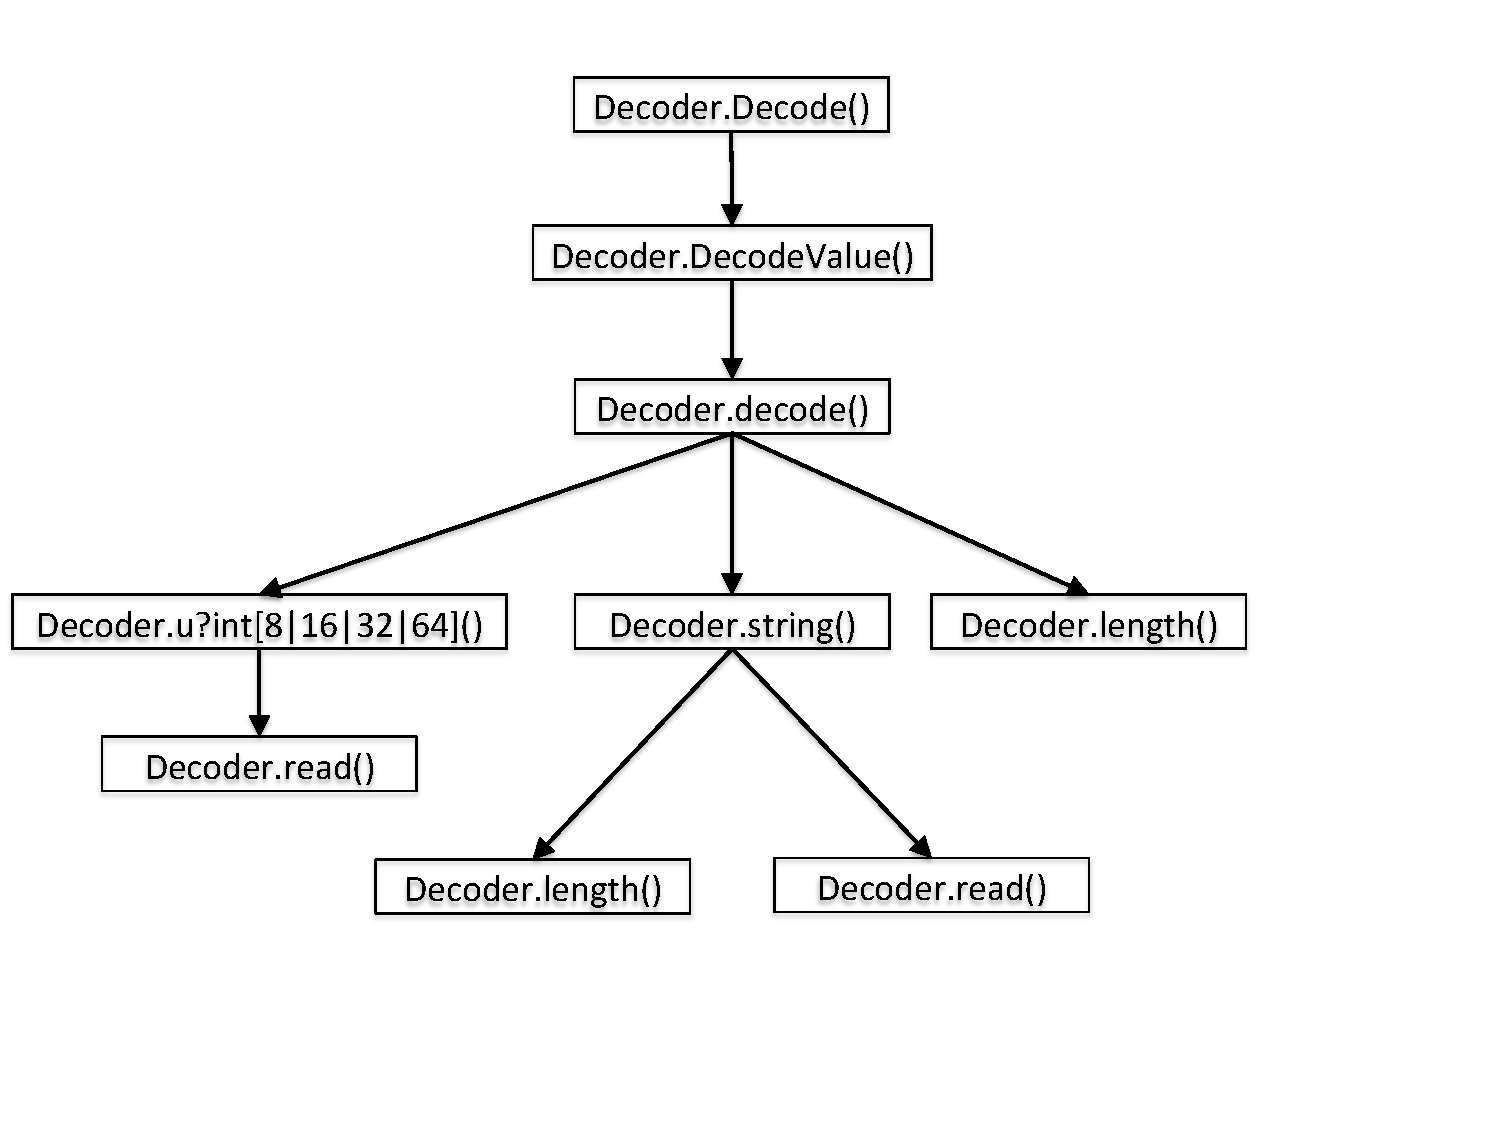
\includegraphics[scale=0.50]{callGraphs/etnDecoderPackage}
\caption{etn.go package: Decoder}
\end{figure}

\begin{figure}[H]
\centering
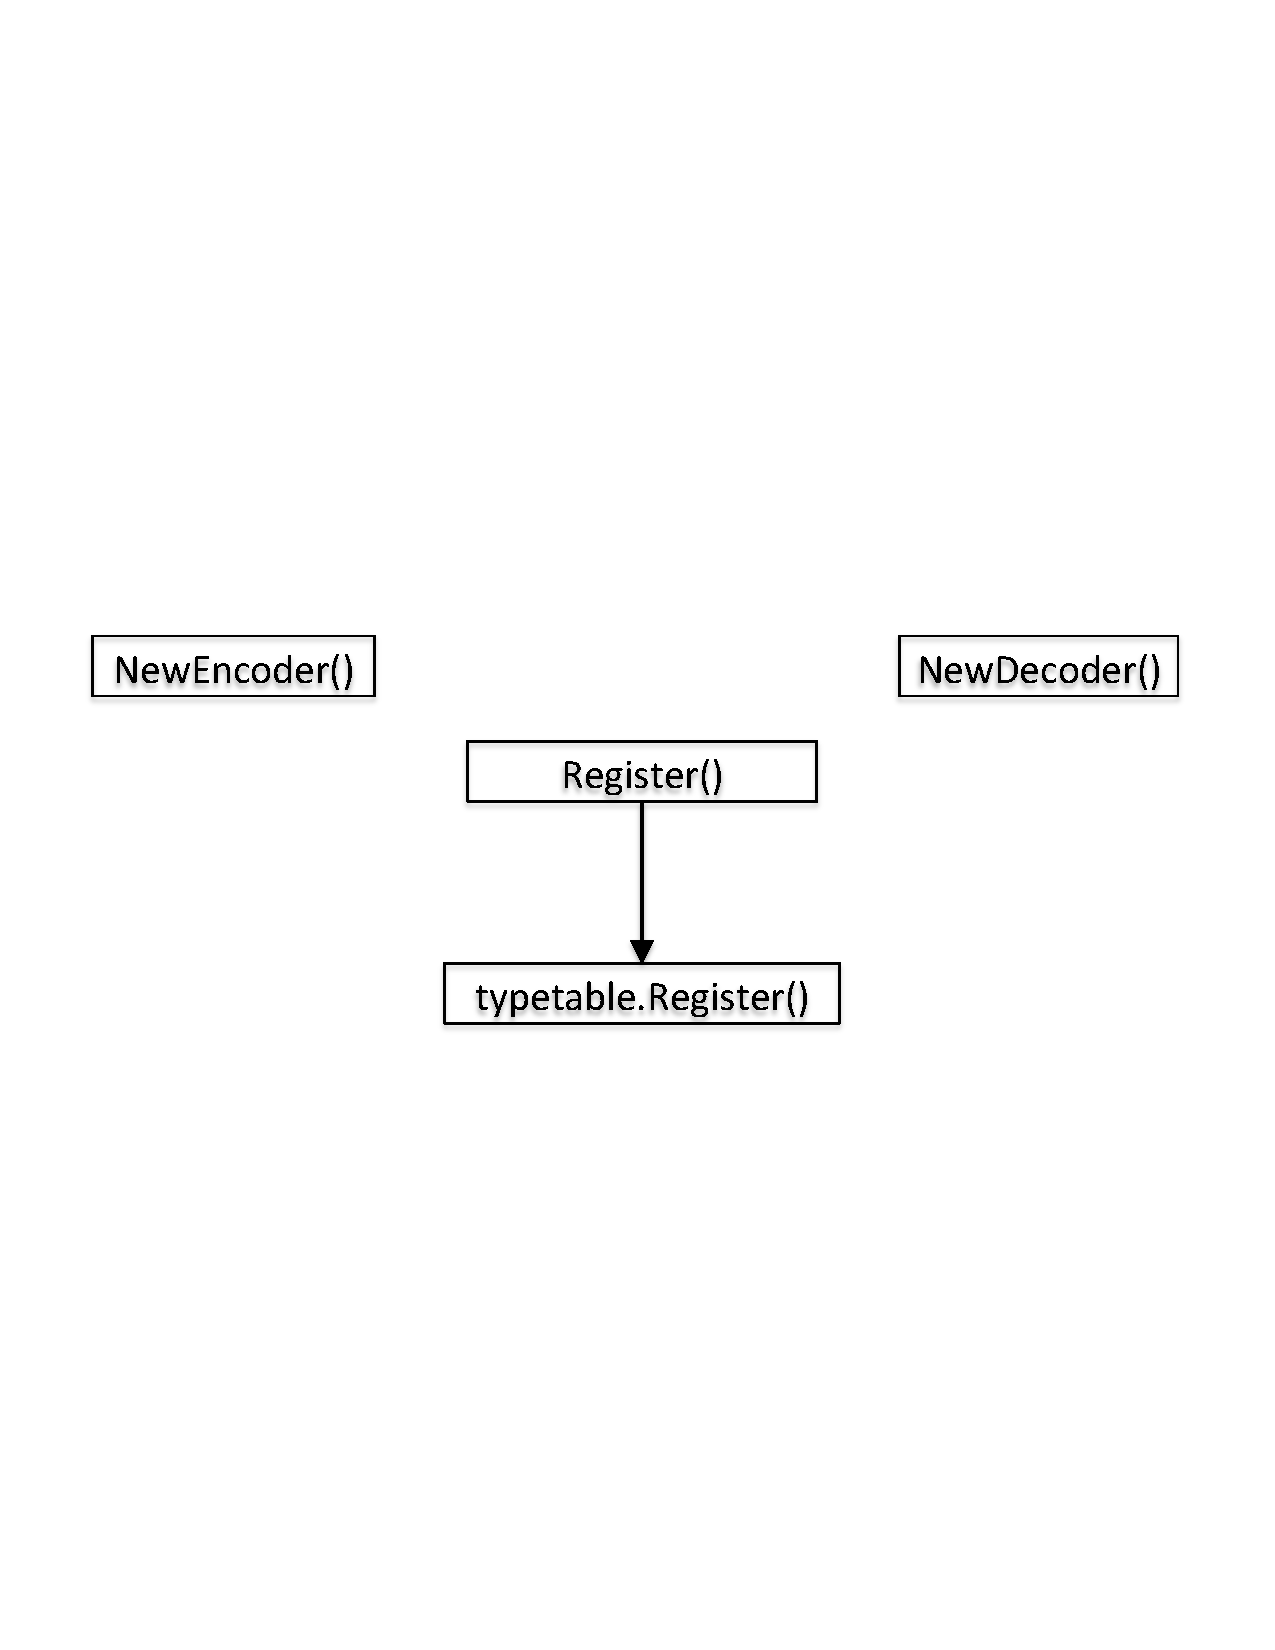
\includegraphics[scale=0.50]{callGraphs/etnConstructorsPackage}
\caption{etn.go package: Constructors}
\end{figure}